
\chapter{Containers}

\subsection*{Virtual Environments}
\begin{center}
    \begin{tabular}{m{7cm}|m{7cm}}
        \textbf{Pros} & \textbf{Cons} \\ \hline
        \begin{itemize}
            \item Reproducible research
            \item Explicit dependencies
            \item Improved engineering collaboration
        \end{itemize} 
        & 
        \vspace{0.5cm}
        \begin{itemize}
            \item Difficulty setting up your environment
            \item Not isolation
            \item Does not always work across different OS
        \end{itemize} 
    \end{tabular}
\end{center}

\subsection*{Virtual Machines}
\begin{center}
    \begin{tabular}{m{7cm}|m{7cm}}
        \textbf{Pros} & \textbf{Cons} \\ \hline
        \begin{itemize}
            \item Full autonomy
            \item Very secure
            \item Isolation
            \item Lower costs
            \item used by all Cloud providers
        \end{itemize} 
        & 
        \vspace{0.5cm}
        \begin{itemize}
            \item Uses hardware in local machine
            \item Not very portable since size of VMs are large
            \item There is an overhead associated with virtual machines 
        \end{itemize} 
    \end{tabular}
\end{center}

\begin{warningblock}[Dependency Hell]
    \begin{itemize}
        \item \textbf{Dependency Hell} is a colloquial term for the frustration of some software users who have installed software packages which have dependencies on specific versions of other software packages.
        \item It is a problem with software dependencies that occurs when a software package is designed to work with particular versions of other software packages.
        \item If a user wants to install a software package that has dependencies on specific versions of other software packages, it can be difficult to resolve these dependencies.
    \end{itemize}
\end{warningblock}

The solution for all these problems is using \textbf{Containers}.

\begin{definitionblock}[Container]
    Informally, a \textbf{container} is a standard unit of software
    that packages up code and all its
    dependencies in processes isolated from
    resources, so the application runs quickly
    and reliably from one computing
    environment to another. Containers creates an isolated
    environment at application level and
    not at server level.
\end{definitionblock}

\newpage
They come with different advantages:
\begin{itemize}
    \item Extremely portable and lightweight
    \item Fully packaged software with all dependencies included
    \item Can be used for development, training and and deployment
    \item Development teams can easily share containers
\end{itemize}

A \textbf{container image} is a lightweight, stand-alone, executable package of a piece of software that includes everything needed to run it: code, runtime, system tools, system libraries, settings. Available for both Linux and Windows based apps, containerized software will always run the same, regardless of the environment.

Container images become containers at runtime and in the case of Docker containers - images become containers when they run on Docker Engine. Available for both Linux and Windows-based applications, containerized software will always run the same, regardless of the infrastructure.   

\begin{figure}[H]
    \centering
    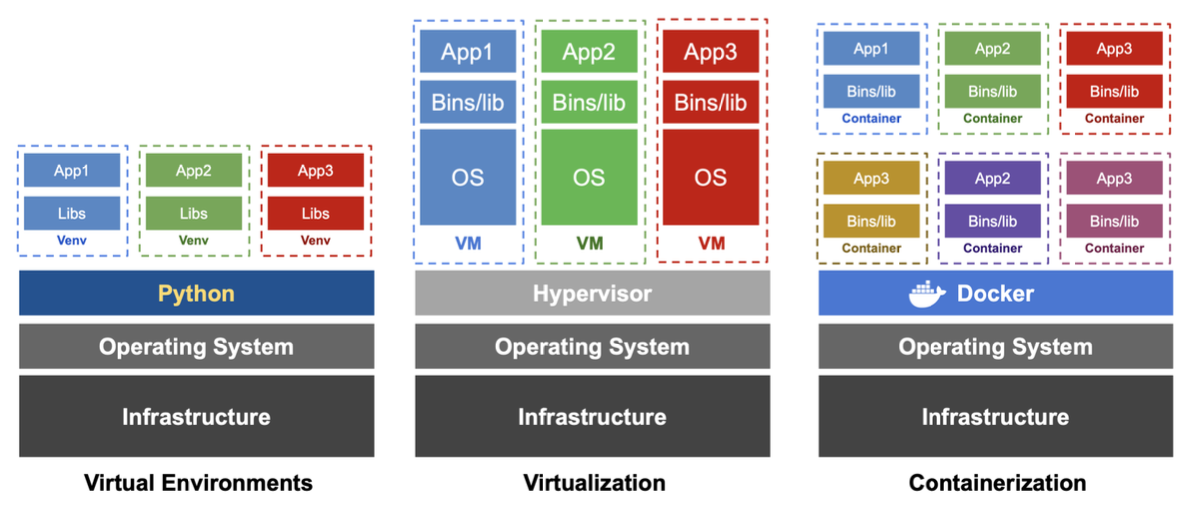
\includegraphics[width=0.8\textwidth]{assets/fig34.png}
    \caption{Comparison between Venvs, VMs and Containers}
\end{figure}

\section{Properties}

\begin{itemize}
    \item \textbf{Isolation}: Containers virtualize CPU, memory, storage, and network resources at
    the OS-level, providing developers with a sandboxed view of
    the OS logically isolated from other applications. Developers, using containers, are
    able to create predictable environments isolated from other applications.
    \item \textbf{Productivity}: enhancement Containers can include software dependencies
    needed by the application (specific versions of
    programming language runtimes, software libraries) guaranteed to be consistent no
    matter where the application is deployed. All this translates to productivity:
    developers and IT operations teams spend less time debugging and diagnosing
    differences in environments, and more time
    shipping new functionality for users.
    \item \textbf{Deployment simplicity}: Containers can be deployed on any machine that has a container runtime installed. This means that developers can build and test containers on their local machine and then deploy them to any environment that supports containers. This makes it easy to move applications between environments, such as from a developer’s laptop to a test environment, or from a test environment to production.
    \item \textbf{Portability}: Containers are portable because they include all of the dependencies needed to run the application. This means that containers can run on any machine that has a container runtime installed, regardless of the underlying infrastructure. This makes it easy to move applications between environments, such as from a developer’s laptop to a test environment, or from a test environment to production.
    \item \textbf{Easy Versioning}: Containers make it easy to version applications. Developers can create a new version of an application by creating a new container image with the new version of the application. This makes it easy to roll back to a previous version of an application if there are any issues with the new version.
    \item \textbf{Scalability}: Containers are lightweight and can be started and stopped quickly. This makes it easy to scale applications up and down based on demand. For example, if an application is experiencing high traffic, additional containers can be started to handle the load. Once the traffic decreases, the additional containers can be stopped.
    \item \textbf{Operational efficiency and reliability}: Containers make it easy to automate the deployment and management of applications. This makes it easy to deploy applications quickly and reliably. Containers can also be used to automate the scaling of applications based on demand. This makes it easy to ensure that applications are always available and responsive.
    \item \textbf{Security}: Containers provide a level of isolation between applications that can help improve security. Containers can be used to run applications in a sandboxed environment that is isolated from other applications. This can help prevent applications from interfering with each other and can help prevent security vulnerabilities from being exploited.
\end{itemize}

The differences with the VMs are:
\begin{itemize}
    \item Containers are more lightweight than VMs
    \item Containers are faster to start and stop than VMs
    \item Containers use less memory than VMs
    \item Containers are more portable than VMs
    \item Containers are easier to manage than VMs
\end{itemize}

You can find a practical example of these differences in my GitHub repository: \href{https://github.com/christianfaccio/cluster_analysis.git}{Cluster Analysis}.

\section{Docker}

\textbf{Docker} is a containerization platform that packages your application and all its
dependencies together in the form of a docker container to ensure that your
application works seamlessly in any environment.

\begin{definitionblock}[Container Engine]
    A \textbf{container engine} is a piece of software that accepts user requests,
    including command line options, pulls images, and from the end user's
    perspective runs the container. It is reponsible for:
    \begin{itemize}
        \item Building images
        \item Running containers
        \item Stopping containers
        \item Removing containers
        \item Managing networks
        \item Managing volumes
    \end{itemize}
\end{definitionblock}

Docker Container is a standardized unit which can be created on the fly to
deploy a particular application or environment. It could be an Ubuntu container,
CentOs container, etc. to full-fill the requirement from an operating system point of
view.

Containers create an isolated environment at application level: each container is a process running including all its children;

Containers underlying (main) technologies:
\begin{itemize}
    \item Linux NAMESPACES: Isolates system resources
    \item Linux CGroups: Limits resources
\end{itemize}

User space refers to all the code in an operating system that lives outside of the kernel.

\begin{figure}[H]
    \centering
    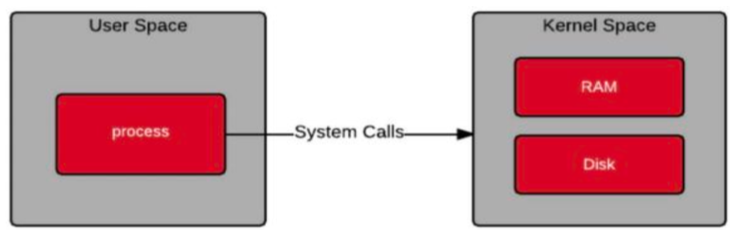
\includegraphics[width=0.8\textwidth]{assets/fig35.png}
    \caption{process Virtualization}
\end{figure}

\subsection{Linux Namespaces}

Linux namespaces provide a mechanism for isolating system resources, enabling
processes within a namespace to have their own view of the system, such as
process IDs,
Namespaces in Linux provide a way to isolate and virtualize system resources, thus
enhancing security by preventing processes in one namespace from directly
interacting with processes in another namespace.
Namespaces increase security by providing a level of isolation that prevents
unintended interactions between processes. This isolation is particularly valuable in
containerization and virtualization scenarios, where multiple applications or
services share the same host system but must be kept separate for security
reasons.

\begin{itemize}
    \item A \textbf{user namespace} has its own set of user IDs and group IDs for assignment to
    processes. In particular, this means that a process can have root privilege within its
    user namespace without having it in other user namespaces.
    \item A \textbf{process ID (PID) namespace} assigns a set of PIDs to processes that are
    independent from the set of PIDs in other namespaces. The first process created in
    a new namespace has PID 1 and child processes are assigned subsequent PIDs. If a
    child process is created with its own PID namespace, it has PID 1 in that namespace
    as well as its PID in the parent process’ namespace.
    \item A \textbf{network namespace} has an independent network stack: its own private routing
    table, set of IP addresses, socket listing, connection tracking table, firewall, and
    other network-related resources.
    \item A \textbf{mount namespace} has an independent list of mount points seen by the processes
    in the namespace. This means that you can mount and unmount filesystems in a
    mount namespace without affecting the host filesystem.
\end{itemize}

Within the parent namespace, there are four processes, named PID1 through PID4. These are normal processes which can all see each other and share resources.

\begin{figure}[H]
    \centering
    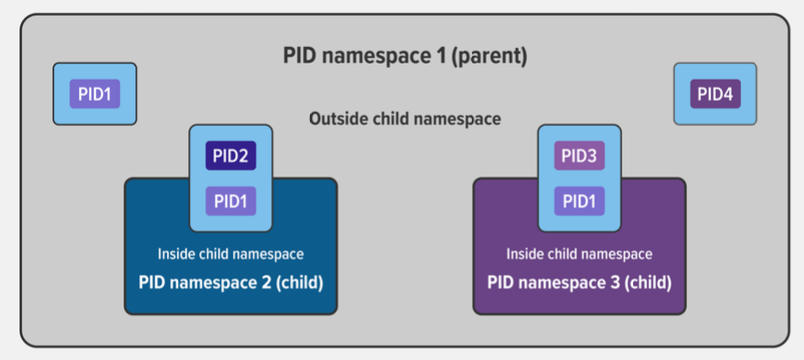
\includegraphics[width=0.6\textwidth]{assets/fig36.png}
    \caption{PIDs}
\end{figure}

To test namespaces, you can use the following commands:
\begin{codeblock}[language=bash]
    # Show all processes
    sudo ps -ef 

    # Show all namespaces
    sudo lsns 

    # Create a new PID namespace
    unshare --fork --pid --mount-proc bash
    
    # Create a new network namespace
    ip netns add test
    ip netns exec test bash
\end{codeblock}

Namespaces are one of the technologies that containers are built on,
used to enforce segregation of resources. We’ve shown how to
create namespaces manually, but container runtimes like Docker, rkt,
and podman make things easier by creating namespaces on your
behalf.

\subsection{Linux CGroups}

A control group (cgroup) is a Linux kernel feature that limits, accounts for, and
isolates the resource usage (CPU, memory, disk I/O, network, and so on) of a
collection of processes.

Main features are:
\begin{itemize}
    \item \textbf{Resource limiting}: Set limits on the amount of resources a group of processes can use.
    \item \textbf{Prioritization}: Give certain groups of processes higher or lower priority.
    \item \textbf{Accounting}: Keep track of the resources used by a group of processes.
    \item \textbf{Control}: Freeze, resume, or kill a group of processes.
\end{itemize}

Kernel uses cgroups to control how much of a given key resource (CPU, memory,
network, and disk I/O) can be accessed or used by a process or set of processes.

\begin{figure}[H]
    \centering
    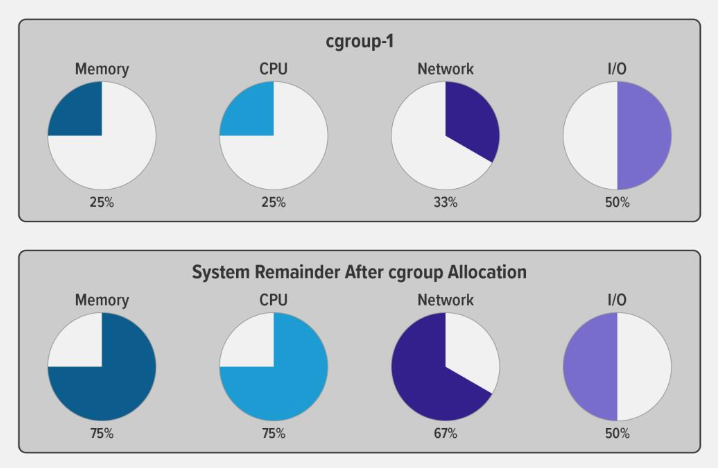
\includegraphics[width=0.8\textwidth]{assets/fig37.png}
    \caption{CGroups}
\end{figure}

You can access cgroups with various tools:
\begin{codeblock}[language=bash]
    # Show all cgroups
    sudo lscgroup

    # Show cgroup hierarchy
    systemd-cgtop
    
    # Create a new cgroup
    sudo cgcreate -g memory:mygroup

    # Set memory limit
    sudo cgset -r memory.limit_in_bytes=1G mygroup

    # Add a process to a cgroup
    sudo cgclassify -g memory:mygroup $PID

    # Control groups can be implemented directly by container engines
    docker run -d --name mycontainer --memory 1g myimage
\end{codeblock}

\subsection{Docker File}

To build a Docker image, you need to create a Dockerfile. A Dockerfile is a text
document that contains all the commands a user could call on the command line to
assemble an image. Using docker build users can create an automated build that 
executes several command-line instructions in succession.

\begin{figure}[H]
    \centering
    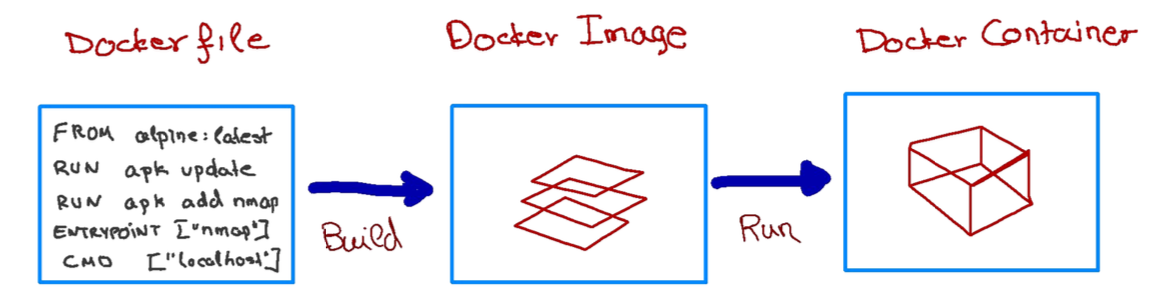
\includegraphics[width=0.8\textwidth]{assets/fig38.png}
    \caption{Dockerfile}
\end{figure}

The Dockerfile has the following structure:
\begin{itemize}
    \item \textbf{FROM}: This instruction in the Dockerfile tells the daemon, which
    base image to use while creating our new Docker image. In the
    example here, we are using a very minimal OS image called alpine
    (just 5 MB of size). You can also replace it with Ubuntu, Fedora,
    Debian or any other OS image.
    \item \textbf{RUN}: This command instructs the Docker daemon to run the given
    commands as it is while creating the image. A Dockerfile can have
    multiple RUN commands, each of these RUN commands create a
    new layer in the image.
    \item \textbf{ENTRYPOINT}:  The ENTRYPOINT instruction is used when you
    would like your container to run the same executable every time.
    Usually, ENTRYPOINT is used in scenarios where you want the
    container to behave exclusively as if it were the executable it's
    wrapping.
    \item \textbf{CMD}: The CMD sets default commands and/or parameters when a
    docker container runs. CMD can be overwritten from the command
    line via the docker run command.
\end{itemize}

\begin{exampleblock}[Dockerfile]
    \begin{codeblock}[language=bash]
        FROM ubuntu:18.04
        RUN apt update
        RUN apt upgrade
        ENTRYPOINT ["echo", "Hello, World!"]
    \end{codeblock}
\end{exampleblock}

You can create multiple containers from the same image, and each container will
have its own isolated environment. You can also create multiple images from the
same Dockerfile, and each image will have its own set of layers.

Docker images are based on layers. Each layer is a set of read-only files that is
created when the image is built. When you run a container from an image, Docker
creates a read-write layer on top of the image layers. This read-write layer is
where the container writes data.

\begin{figure}[H]
    \centering
    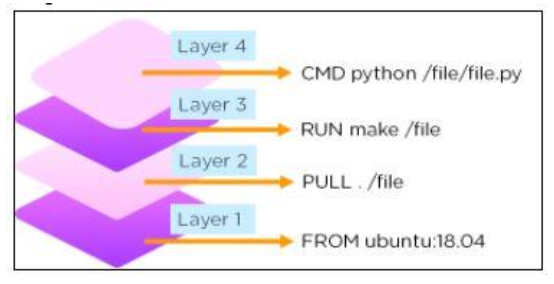
\includegraphics[width=0.5\textwidth]{assets/fig39.png}
    \caption{Docker Layers}
\end{figure}




